\documentclass [11pt, a4paper, oneside] {article}
\usepackage {amsmath}
\usepackage {geometry}
\geometry{left=2.5cm,right=2.5cm}
\usepackage {amssymb}
\usepackage {graphicx}
\usepackage {pythonhighlight} 
\usepackage{multirow}
\linespread{1.5}
\usepackage{color}
\author {Yue Wang, A53102167}
\title {CSE255 Homework2 Answer}
\begin {document}
\maketitle
\section *{PCA Clustering}
\subsection *{1}
The reconstruction error is 113183.43370488819.
\begin{python}
def reconsError(X, XTrans):
    reconsError = 0;
    for i in xrange(len(X)):
        for j in xrange(len(X[i])):
            reconsError = reconsError + (X[i][j]-XTrans[i][j])**2
    return reconsError
meanVector = []
for i in xrange(len(X[0])):
    meanVector.append(numpy.mean(map(lambda x: x[i], X)))
reconsError(X, XMeanCompress)
\end{python}
\subsection *{2}
The PCA components are:\\
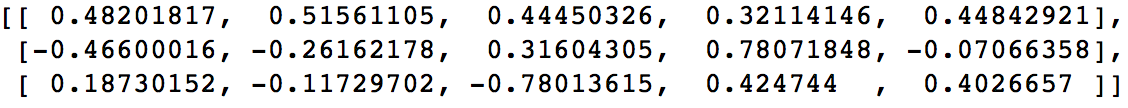
\includegraphics[height=1cm]{pca.png}\\
And the reconstruction error(MSE) is: 0.23428831021990038\\
\begin{python}
pca = PCA(n_components=3)
pca.fit(X)
pca.components_
XTrans = pca.transform(X)
XTransBack = pca.inverse_transform(XTrans)
reconsError(X, XTransBack)/len(X)
\end{python}
\subsection *{3}
The sizes of the last two clusters are: 9 and 491. Their's centroids are \[1.66666667,  1.83333333,  2.16666667,  2.72222222,  1.88888889\] and  \[4.02851324,  3.91955193,  3.84114053,  3.92973523,  3.83706721\] respectively.
\begin{python}
def cluster(X):
    dists = [[0] * len(X) for row in xrange(len(X))]
    for i in xrange(len(X)):
        for j in xrange(len(X)):
            if i != j:
                dists[i][j] = (X[i][len(X[i])-1]-X[j][len(X[j])-1]).dot(X[i][len(X[i])-1]-X[j][len(X[j])-1])
            else:
                dists[i][j] = sys.float_info.max
    clu1 = X[numpy.where(dists==numpy.min(dists))[0][0]]
    clu2 = X[numpy.where(dists==numpy.min(dists))[1][0]]
    clu = clu1[0:-1] + clu2[0:-1]
    clu.append(numpy.mean(clu, axis=0))
    X.remove(clu1)
    X.remove(clu2)
    X.append(clu)
    print "clu1:"
    print clu1
    print "clu2:"
    print clu2
    return X
XCluster = X[0:500]
XCluster = [[x] for x in XCluster]
for x in XCluster:
    x.append(numpy.mean(x, axis=0))
while len(XCluster) > 2:
    cluster(XCluster)
    print len(XCluster)
print len(XCluster)
print len(XCluster[0])-1
print len(XCluster[1])-1
\end{python}
\subsection *{4}
The reconstruction error(MSE) is: 1.2550355284000967\\
\begin{python}
XOrigin = X[0:500]
XRed = []
for x in XOrigin:
    if x in XCluster[0][0:-1]:
        XRed.append(XCluster[0][len(XCluster[0])-1])
    else:
        XRed.append(XCluster[1][len(XCluster[1])-1])
reconsError(XOrigin, XRed)/len(XOrigin)
\end{python}
\section *{Community Detection}
\subsection *{1}
There are 3 connected components in the graph and there are 40 nodes in the largest connected components.\\
\begin{python}
import networkx as nx
import math
import copy
from operator import itemgetter, attrgetter
G = nx.Graph()
with open('./egonet.txt', 'r') as file:
    for line in file:
        line = line.strip().split(' ')
        G.add_edge(line[0], line[1])
components = nx.connected_components(G)
gNodes = list(sorted(components, key=len, reverse=True)[0])
g = G.subgraph(list(gNodes))
print g.number_of_nodes()
nodes1 = sorted(g.nodes(),reverse=True)[0:len(g.nodes())/2]
nodes2 = sorted(g.nodes(),reverse=True)[len(g.nodes())/2:]
\end{python}
\subsection *{2}
The normalized-cut cost is 0.42240587695133147\\
\begin{python}
def cut(nodesList, nodes, g):
    res = 0.0
    for i in nodesList:
        g1 = g.subgraph(i)
        leftNodes = []
        for x in g.nodes():
            if x not in i:
                leftNodes.append(x)
        g2 = g.subgraph(leftNodes)
        numEdgesCrossed = (g.number_of_edges()-g1.number_of_edges()-g2.number_of_edges())*1.0
        res = res + numEdgesCrossed/sum(g.degree(i).values())
    return res/len(nodesList)
g1 = g.subgraph(nodes1)
g2 = g.subgraph(nodes2)
numEdgesCrossed = (g.number_of_edges()-g1.number_of_edges()-g2.number_of_edges())*1.0
d1 = sum(g1.degree().values())
d2 = sum(g2.degree().values())
cut([nodes1, nodes2], g.nodes(), g)
\end{python}
\subsection *{3}
The split is:\\
1: '893', '889', '888', '886', '884', '882', '878', '876', '864', '863', '861', '825', '729', '804'\\
2: '819', '811', '810', '805', '803', '800', '798', '774', '772', '769', '753', '747', '745', '719', '713', '708', '703', '697', '828', '823', '830', '840', '880', '890', '869', '856'\\
The cut cost is 0.0981704596162\\
\begin{python}
while True:
    lastcost = cost
    costs = {}
    for i in g.nodes():
        nodesTmp1 = copy.deepcopy(nodes1)
        nodesTmp2 = copy.deepcopy(nodes2)
        if i in nodesTmp1:
            nodesTmp1.remove(i)
            nodesTmp2.append(i)
        else:
            nodesTmp2.remove(i)
            nodesTmp1.append(i)
        costs[i] = cut([nodesTmp1, nodesTmp2], g.nodes(), g)
    minimum = sorted(costs.items(), key=itemgetter(1, 0))[0]
    node = minimum[0]
    cost = minimum[1]
    if lastcost<cost:
        break
    if node in nodes1:
        nodes1.remove(node)
        nodes2.append(node)
    else:
        nodes2.remove(node)
        nodes1.append(node)
    lastcost = cost
    print cost
print nodes1
print nodes2
\end{python}
\subsection *{4}
The 4 communities are:\\
1: '889', '888', '886', '882', '878', '876', '804', '729', '863', '861'\\
2: '864', '825', '884', '893'\\
3: '811', '798', '869', '769', '890', '708', '753'\\
4: '747',
  '745',
  '719',
  '713',
  '703',
  '697',
  '819',
  '823',
  '830',
  '840',
  '805',
  '880',
  '803',
  '828',
  '810',
  '772',
  '800',
  '774',
  '856'\\
 The cost is 0.280598888492.\\
 \begin{python}
 g = G.subgraph(list(gNodes))
nodes1 = sorted(g.nodes(),reverse=True)[0:len(g.nodes())/4]
nodes2 = sorted(g.nodes(),reverse=True)[len(g.nodes())/4:len(g.nodes())/2]
nodes3 = sorted(g.nodes(),reverse=True)[len(g.nodes())/2:3*len(g.nodes())/4]
nodes4 = sorted(g.nodes(),reverse=True)[3*len(g.nodes())/4:]
nodesList = [nodes1, nodes2, nodes3, nodes4]
cost = 100
while True:
    lastcost = cost
    costs = []
    
    for i in g.nodes():
        num = 0;
        for j in xrange(len(nodesList)):
            if i in nodesList[j]:
                num = j
                break
        nodesTmp = []
        for j in nodesList:
            nodesTmp.append(copy.deepcopy(j))
        nodesTmp[num].remove(i)
        for j in xrange(len(nodesList)):
            if j == num:
                localcost.append([10000, min(nodesList[j]), num, j, i])
            else:
                tmptmp = copy.deepcopy(nodesTmp[j])
                nodesTmp[j].append(i)
                costs.append([cut(nodesTmp, g.nodes(), g), min(tmptmp), num, j, i])
                nodesTmp[j].remove(i)
        
    minimum = sorted(costs, key=itemgetter(0, 4, 2))[0]
    cost = minimum[0]
    node = minimum[4]
    fromG = minimum[2]
    toG = minimum[3]
    if lastcost < cost:
        break
    nodesList[fromG].remove(node)
    nodesList[toG].append(node)
    lastcost = cost
    print cost
print nodesList
\end{python}
\end{document}
